\documentclass{article}
\usepackage{amsthm}
\usepackage{amsmath}
\usepackage{bm}
\usepackage{makeidx}
\usepackage{tikz}
\usepackage{physics}
\usepackage{cite}
\usetikzlibrary{arrows.meta}

%\usepackage[
%  top=1.25in,
%  bottom=1.25in,
%  left=1.25in,
%  right=1.25in,
%  bindingoffset=0.25in,
%  heightrounded,
%]{geometry}

\def\lsqb{\left[}
\def\rsqb{\right]}
\def\sqb#1{\lsqb #1 \rsqb}
\def\xsig{x\sqb{n}}
\def\ysig{y\sqb{n}}

\makeindex
\begin{document}
\title{The DSP Cookbook}
\date{October 2017}
\author{Pelle Juul Christensen}
\maketitle
\tableofcontents

\section{Theory}
\subsection{Sine Wave}
\index{Sine waves}
\index{Sin}
\index{Cos}

The general equation of is
\begin{equation}
    A\sin(2\pi t f + \theta),
\end{equation}
where
\begin{description}
    \item[$A$] is the amplitude of the wave.
    \item[$\sin$] is the $\sin$ function.
    \item[$2\pi$] normalizes the period of the $\sin$ function to $1$.
    \item[$t$] is time.
    \item[$f$] is the frequency of the wave.
    \item[$\theta$] is the phase offset of the wave.
\end{description}

The $\sin$ and $\cos$ functions are defined using the unit circle. Given a variable $t$ we go $t$ radians along the unit circle \footnote{A unit circle is simply a circle with a radius of 1}. The point at $t$ radians will have coordinates $(\cos(t), \sin(t))$ --- $\cos(t)$ is the projection of the point onto the x-axis, $\sin(t)$ is the projection onto the y-axis.

\begin{figure}[h]
\centering
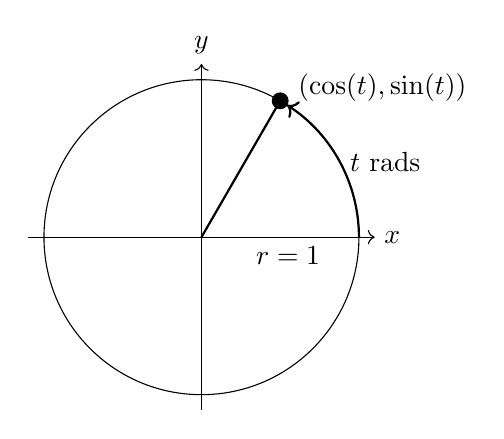
\begin{tikzpicture}[scale=2, domain=0:3]
    \draw (0, 0) circle [radius=1.0];
    \draw [->] (-1.1, 0) -- (1.1, 0) node [right] {$x$} node[pos=0.75, below] {$r=1$};
    \draw [->] (0, -1.1) -- (0, 1.1) node [above] {$y$};
    \draw[thick] (0, 0) -- (60:1) node[pos=1.1, right] {$(\cos(t), \sin(t))$};
    \filldraw (60:1) circle [radius=0.05];
    \draw[thick] [->] (1, 0) arc (0:57:1) node[pos=0.5,right] {$t$ rads};
\end{tikzpicture}
\end{figure}

\index{period}
Sinusoids have a period of $2 \pi$ (a full arc), thus if we multiply $t$ by $2\pi$ to get $\sin(2 \pi t)$, we will get a period of $1$. If $t$ is time in seconds, we will have one period per second.

To get more or less periods per second we multiply $t$ by that amount. For example $\sin(2 \pi t 440)$ has 440 periods per second.

\index{Frequency}
\index{Hertz}
\index{Hz|see {Hertz}}
Periods per second is measured in $Hertz$ which has the unit $1/s$, which is also called the frequency of a wave. To calculate the period of a sine wave at a specific frequency $f$, you use $1/f$, e.g. a sine wave at $440Hz$ will have a period of $1/f=0.002s$.

\index{Phase}
We can change the starting point of a wave by adding a phase component. A $\sin$ wave with a phase of $\pi/2$ is equivalent to a $\cos$ wave. The phase component is usually written as $\theta$

\index{Amplitude}
A sine wave swings between $-1$ and $1$. To increase or decrease the amplitude, we multiply with a gain factor $A$.

\subsection{Phasors}
\index{Phasor}
A \textit{Phasor} is a complex sinusoid defined my Euler's equation
\begin{equation}
    e^{jx} = \cos(x) + j\sin(x),
\end{equation}
such that we have
\begin{align}
    \cos(x) = \Re{e^{jx}}\\
    \sin(x) = \Im{e^{jx}}
\end{align}

\subsection{Digital Signals}
\index{Digital signals}
\index{Sampling rate}
\index{Sampling period}
Unlike real-world \textit{analog} signals, which are continuous, digital signals are represented by discrete numbers at specific points in time --- a list of numbers. Each number is separated by some amount of time called the \textit{sampling rate}.

If we wish to convert a analog signal to a digital one, we must sample it. This is done by measuring the analog signal one time each \textit{sampling period} ($1/samplerate$). Given the analog signal $x(t)$ then we have the digital signal
\begin{equation}
    \xsig = x(nT),
\end{equation}
where $T$ is the sampling period and $n$ is the \textit{sample index}. Notice that it is convention to use square brackets for discrete signals and parentheses for continuous signals.

\index(ADC)
\index{Quantization}
If we are measuring a real-world signal, we will use an \textit{Analog to Digital Converter (ADC)}. Since computers only have a finite amount of memory, we will need to choose how precise our measurements will be. If we represent out sample with $b$ bits then we will have $2^b$ levels to work with. The process of rounding our sample to the nearest representable number is called \textit{quantization}

\subsection{DSP Systems}
\index{System}
A DSP system (or just "a system") is a computer program --- an algorithm --- which takes one or more digital signal and returns one or more digital signals.

\subsection{Causal Systems}
In systems with memory, we need to agree on what should happen when $n < 0$. Usually we will use $x\left[n\right] = 0 \text{ for } n < 0$. Such a system is said to be \textit{cusal}.

If we have a system where $x\left[n\right] \neq 0 \text{ for } n < 0$, then the system is said to be \textit{non-causal}.

\subsection{Difference Equations}
The general form of a difference equation is

\begin{equation}
\begin{split}
    y\sqb{n} = a_1 y\sqb{n - 1} + a_2 y\sqb{n-2} + \dots + a_N y\sqb{n-N} + \\
        b_0 x\sqb{n} + b_1 x\sqb{n - 1} + b_2 x\sqb{n - 2} + \dots + b_L\sqb{n - L}.
\end{split}
\end{equation}

Also written as

\begin{equation}
    y\sqb{n} = \sum_{k=1}^N a_k y\sqb{n - k} + \sum_{k=0}^L b_k x\sqb{n - k}.
\end{equation}

Where the $y\sqb{\cdot}$ components determine the recursive (feedback) characteristic, and the $x\sqb{\cdot}$ components the non-recursive characteristic.

\subsection{Linear Time-Invariant System}
\index{Linear Time-Invariant System}
\index{LTI|see {Linear Time-Invariant System}}

A system $T(x\sqb{n})$ is \textit{linear time-invariant} (LTI) is it is both linear and time-invariant.

A system is linear if it supports the scalability property \index{Linearity property}
\begin{equation}
    T(\alpha \xsig) = \alpha T(\xsig).
\end{equation}
As well as the superposition property \index{Superposition property}
\begin{gather}
    T(x_3\sqb{n}) = T(x_1\sqb{n} + x_2\sqb{n}) =  T(x_1\sqb{n}) + T(x_2\sqb{n}), 
\end{gather}
where $x_3\sqb{n} = x_1\sqb{n} + x_2\sqb{n}$.

A system is time-invariant if it meets the condition
\index{Time-invariant}
\begin{equation}
    x\sqb{n - L} = y\sqb{n - L}
\end{equation}
for some delay $L$ --- a delay in the input signal will cause a corresponding delay in the output signal.

A system is LTI if all of its subcomponents are LTIs.

\subsection{Impulse Response}
\index{Impulse response}
An impulse is a short spike in amplitude. The ideal impulse signal is defined by

\begin{equation}
    \delta\sqb{n} =
        \begin{cases}
            1, & \text{if } n = 0 \\
            0, & \text{otherwise}
        \end{cases}.
\end{equation}

The \textit{impulse response} of a system is how it reacts to an input of $\xsig = \delta\sqb{n}$. In this
case the ouput of the system is normally denoted $h\sqb{n}$.

LTI systems can be described completely by their impulse responses. To obtain the output of a system based on an impulse response, one should convolute the input signal with the impulse response
\begin{equation}
    T(\xsig) = \xsig * h_T\sqb{n}.
\end{equation}

\index{Finite impulse repsonse}
\index{FIR|see {Finite impulse repsonse}}
A system has \textit{finite impulse response} (FIR) if it does not contain any recursive components. In that case the impulse response is determined by
\begin{equation}
    h\sqb{n} = T(\delta\sqb{n}) = \sum_{k = 0}^L b_k \delta\sqb{n - k}.
\end{equation}
The impulse response of FIR systems will always converge to zero.

\index{Infinte impulse response}
\index{IIR|see {Infinte impulse response}}
A system has \textit{infinte impulse reponse} (IIR) if it contains recursive components. In that case the impulse response is determined by
\begin{equation}
    h\sqb{n} = T(\delta\sqb{n}) = \sum_{k=1}^N a_k h\sqb{n - k} + \sum_{k = 0}^L b_k \delta\sqb{n - k}.
\end{equation}
\index{Stability}
\index{Stable}
\index{Unstable}
Some IIR systems will converge to a state of near-zero. Such systems are said to be \textit{stable}. IIR systems can also be \textit{unstable}, which means that their output will be non-convergent (i.e. blow up).

\subsection{Convolution}
\index{Convolution}
The \textit{convolution} of two signals $\xsig$ and $h\sqb{n}$ is defined as
\begin{equation}
    \xsig * h\sqb{n} = \sum_{m = -\infty}^{m = \infty} x\sqb{n - m}h\sqb{m}.
\end{equation}

In reality $m$ will be bounded by the sizes of the signals. If $\xsig$ has size $N$ and $h\sqb{n}$ size $M$, then $m$ should be within $0$ and $M$, since no samples is defined before $0$, and no smaples in $h\sqb{x}$ are defined after $M$. The equation is then
\begin{equation}
    \xsig * h\sqb{n} = \sum_{m = 0}^{M} x\sqb{n - m}h\sqb{m}.
\end{equation}
The result will be defined for $n$ in $0 \leq n < N + M$.

Convolution is commutative, meaning that
\begin{equation}
    \xsig * h\sqb{n} = h\sqb{n} * \xsig.
\end{equation}
It is also associative, which means that
\begin{equation}
    g\sqb{x} * (\xsig * h\sqb{n}) = (g\sqb{x} * \xsig) * h\sqb{n},
\end{equation}
as well as distributive
\begin{equation}
    g\sqb{x} * (\xsig + h\sqb{n}) = (g\sqb{x} * \xsig) + (g\sqb{x} *  h\sqb{n}).
\end{equation}

\subsection{Digital Frequency}
\index{Digital frequency}
Digital frequency is defined as
\begin{equation}
    \theta = 2\pi f T,
\end{equation}
where $f$ is the frequency in $Hz$ and $T$ is the sampling period. This means that $\theta=0$ denotes DC, $\theta=\pi$ the Nyquist frequency ($1/2 * samplerate$), and $\theta=2\pi$ the sampling frequency.

\subsection{Frequency Response}
\index{Frequency response}
\index{Bode diagram}
The frequency response of a system describes how it responds to signals of a specific frequency, in terms of magnitude and phase. The frequency response of a system is usually shown as a plot with frequency on the x-axis and amplitude on the y-axis. If the plot is presented with a logarithmic frequency scale, it is sometimes called a \textit{Bode} diagram.

Using the equation
\def\hfun{H(e^{j\theta})}
\begin{equation}
    \hfun = \frac{\sum_{k=0}^{L} b_k e^{-j\theta k}}{\sum_{k=1}^{N} a_k e^{-j\theta k}},
\end{equation}
we get a complex number which describes the phase and magnitude response for a signal at the digital frequency $\theta$. The magnitude $\|\hfun\|$ is the gain at that frequency. The angle $\angle \hfun$ is the \textit{phase shift} at that frequency.

The $\hfun$ term is derived by first selecting the input signal
\begin{equation}
    \xsig = e^{j\theta n},
\end{equation}
and then convolving with the impulse response of our system
\def\convsum{\sum_{m=-\infty}^{\infty}}
\begin{align}
    \ysig &= \convsum h\sqb{m} x\sqb{n-m} = \convsum h\sqb{m} e^{j\theta(n-m)} \\
          &= e^{j\theta(n)} \convsum h\sqb{m} e^{j\theta m} = \xsig \convsum h\sqb{m} e^{j\theta m} \\
          &= \xsig \hfun,
\end{align}
so we have
\begin{equation}
    \hfun = \convsum h\sqb{m} e^{j\theta m},
\end{equation}
and since
\begin{equation}
    \ysig = \xsig \hfun,
\end{equation}
we have
\begin{equation}
    \hfun = \frac{\ysig}{\xsig}
\end{equation}

To get to our final definition of $\hfun$ we first not that
\begin{align}
    \ysig &= \convsum h\sqb{m} x\sqb{n-m} \\
    \ysig &= \xsig \hfun = e^{j\theta n} \hfun
\end{align}
And then rearranging
\begin{align}
    e^{j\theta n} \hfun &= \sum_{k=1}^{N} a_k e^{j\theta (n-k)} \hfun + \sum_{k=0}^{L} b_k e^{j\theta(n-k)} \\
    e^{j\theta n} \hfun &= e^{j\theta n} \left( \sum_{k=1}^{N} a_k e^{-j\theta k} \hfun + \sum_{k=0}^{L} b_k e^{-j\theta k} \right)\\
    \hfun &= \sum_{k=1}^{N} a_k e^{-j\theta k} \hfun + \sum_{k=0}^{L} b_k e^{-j\theta k} \\
    1 &= \sum_{k=1}^{n} a_k e^{-j\theta k} + \frac{\sum_{k=0}^{L} b_k e^{-j\theta k}}{\hfun} \\
    1 - \sum_{k=1}^{n} a_k e^{-j\theta k} &= \frac{\sum_{k=0}^{L} b_k e^{-j\theta k}}{\hfun} \\
    \frac{1 - \sum_{k=1}^{n} a_k e^{-j\theta k}}{\sum_{k=0}^{L} b_k e^{-j\theta k}} &= \frac{1}{\hfun}\\
    \hfun &= \frac{\sum_{k=0}^{L} b_k e^{-j\theta k}}{1 - \sum_{k=1}^{n} a_k e^{-j\theta k}} \label{eq:frequency_response}
\end{align}

\subsection{Z-transform}
\index{Z-transform}
The $z$-transform is a way of analysing the frequency response of a system. It is defined by
\begin{equation}
    Z(\xsig) = X(z) = \sum_{n=-\infty}^{\infty} \xsig z^{-n},
\end{equation}
and has the shifting property
\begin{equation}
    Z(x\sqb{n-m}) = z^{-m} \sum_{n=-\infty}^{\infty} x\sqb{n} z^{-n} = z^{-m} X(z).
\end{equation}

If we apply the $z$-transform to the general difference equation we get
\begin{align}
    \ysig = \sum_{k=1}^N a_k y\sqb{n-k} + \sum_{k=0}^L b_k x\sqb{n-k} \\
    Y(z) = \sum_{k=1}^N a_k z^{-k} Y(z) + \sum_{k=0}^L b_k z^{-k} X(z) \\
\end{align}
from which we arrive at
\index{Transfer function}
\begin{equation}
    \label{eq:ztransform}
    \frac{Y(z)}{X(z)} = \frac{\sum_{k=0}^L b_k z^{-k}}{1 - \sum_{k=1}^N a_k z^{-k}},
\end{equation}
which is called the \textit{transfer function}. Note that setting $z = e^{j\theta}$ makes the above equation equal to the frequency response(Eq. \ref{eq:frequency_response}).

\index{Poles}
\index{Zeros}
We use the above equation to solve for \textit{poles} and \textit{zeros} of the system. The zeros are found by solving the equation
\begin{equation}
    \sum_{k=0}^L b_k z^{-k} = 0,
\end{equation}
which is the numerator of Eq. \ref{eq:ztransform} --- when this is zero, the system response will be zero.

To find the poles, we solve for the numerator like
\begin{equation}
    1 - \sum_{k=1}^N a_k z^{-k} = 0,
\end{equation}
which gives us the places where the ratio explodes into infinity.

In reality the poles and zeros will cancel each other out by different amounts based on the input frequency. Therefore, the response will seldom actually be zero or infinity.

\section{Recipes}
\subsection{Biquad Filters}
\index{Biquad filter}
\index{Second order filter}
Biquad filters are a general form of second-order two pole, two zeros filters. They have the difference equation
\begin{equation}
    H(z) = \frac{b_0 + b_1 z^{-1} + b_2 z ^{-2}}{1 + a_1 z_{-1} + a_2 z_{-2}}.
\end{equation}

If we multiply this by $z^2 / z^2$ we get 
\begin{equation}
    H(z) = \frac{b_0 z^2 + b_1 z + b_2}{z^2 + a_1 z + a_2 z},
\end{equation}
and see that both the numerator and denominator are quadratic equations, hence the name.

Biquad filters can be used to implement many common types of filter including low-pass, high-pass, bandpass, band-reject and all-pass.

For calculating the coefficients of these filters we will need
\begin{equation}
    K = \tan (\pi f_c / f_s),
\end{equation}
where $f_c$ is the filter center frequency and $f_s$ is the sample rate.

\subsubsection{Low-pass Filter}
\index{Low-pass filter}
Low-pass biquad filters are designed by selecting a cutoff frequency $f_c$, and a $Q$ factor which controls the gain around $f_c$.
When $Q = 1/\sqrt 2$ the filter will be flat around $f_c$ --- values above or below will cause amplification or attenuation.

The coefficients are then calculated by:
\begin{align}
    b_0 &= \frac{K^2Q}{K^2Q + K + Q}\\
    b_1 &= \frac{2K^2Q}{K^2Q + K + Q}\\
    b_2 &= b_0\\
    a_1 &= \frac{2Q(K^2 - 1)}{K^2Q + K + Q}\\
    a_2 &= \frac{K^2Q - K + Q}{K^2Q + K + Q}
\end{align}
\cite{Zolzer:2011}

\section{References}
\bibliography{dsp-cookbook}{}
\bibliographystyle{apalike}

\printindex
\end{document}
